\chapter{User Manual}

\section{About}

This chapter contains instructions for installing and using the OKSE Message Broker. The intended users are primarily researchers working with collaborative networking.

\section{Requirements}

OKSE Message Broker requires a Java Runtime Environment (hereby denoted as JRE) version 8 update 31 or newer, to be able to run. The latest available update is always recommended. 

The system was developed and tested on Windows, Debian Linux and OS X. It should be possible to run on all platforms with JRE installed. 

In addition to JRE, OKSE requires a network connection to be able to send and receive messages. It does not require Internet on the connection. 

\section{Installation}

The following sections describes how to download and run OKSE. Apart from JRE, no other additional configuration should be necessary.

\subsection{Java Runtime Environment}

As previously stated, OKSE Message Broker requires a JRE 8. The broker is developed and tested exclusively with this version. The software is available for free from Oracle.com\footnote{\url{http://www.oracle.com/technetwork/java/javase/downloads/jre8-downloads-2133155.html}}.

If you are using a UNIX-based system like Linux or OS X, you must remember to add Java to your path variable. Entering the following commands in a terminal should most likely work: \verb!export JAVA_HOME=<PATH-TO-JRE>! If you have to add Java to the path in Windows, open up a command line window(cmd.exe). type in  \verb!path %path%;<PATH-TO-JRE>!.
The variable can also be accessed and modified through the "Environmental variables" tab in the advanced system settings.

\subsection{Download software}

Download the latest version of OKSE Message Broker from [URL HERE].
The file can placed in an appropriate place in the file system. For example: \verb!$HOME/okse/! on UNIX-based systems, and \verb!C:\Program Files\okse\! on Windows.

\subsection{Running the software}

On Windows, the broker can be started by double-clicking on the .jar-file. On UNIX-based systems and Windows alike, the broker could be started by running the command: \verb!java -jar <PATH-TO-JAR-FILE>/<JAR-FILE>.jar! from the command line or terminal.

See section \ref{sec:inital-login} for information about accessing the administration panel.

\section{Configuration}

After the initial start up of OKSE Message Broker, there is created a folder named \verb!config! in the same location as the .jar-file. This folder contains three configuration files with the default configuration:

\begin{itemize}
\setlength{\itemsep}{0cm}%
\item okse.properties
\item log4j.properties
\item topicmapping.properties
\end{itemize}

\noindent See section \ref{sec:configuration-files} for detailed information about all the possible settings.

\section{Inital login}
\label{sec:inital-login}

After installation and the first launch, the OKSE Admin Console can be accessed using a web-browser. By default, the admin console is accessible from \verb!localhost:8080!. Both the host and port can be changed in the okse.properties (see section \ref{sec:configuration_okse.properties}). To log in for the first time, use \verb!admin! and \verb!password! as respectively username and password. To increase the security, it is recommended that this is changed immediately after the inital login. 

\begin{itemize}
\setlength{\itemsep}{0cm}%
\item Default host and port for admin console: \verb!localhost:8080!
\item Default username and password: \verb!admin! and \verb!password!
\end{itemize}

\section{Admin Console}
The OKSE Admin Console provides information about OKSE and it's operation enviroment. It also gives access to configure OKSE. The interface have information sorted in six panes, the Main pane, the Topic pane, the Subscribers pane and the Configuration pane.

\subsection{The Main pane}
The Main pane is an overview of the broker's status, system, the operating environment, and the interfaces the different protocol servers are bound to. It is also possible to stop and start the protocol servers from the interface section.

\begin{center}
  \begin{figure}[ht!]
    \makebox[\textwidth]{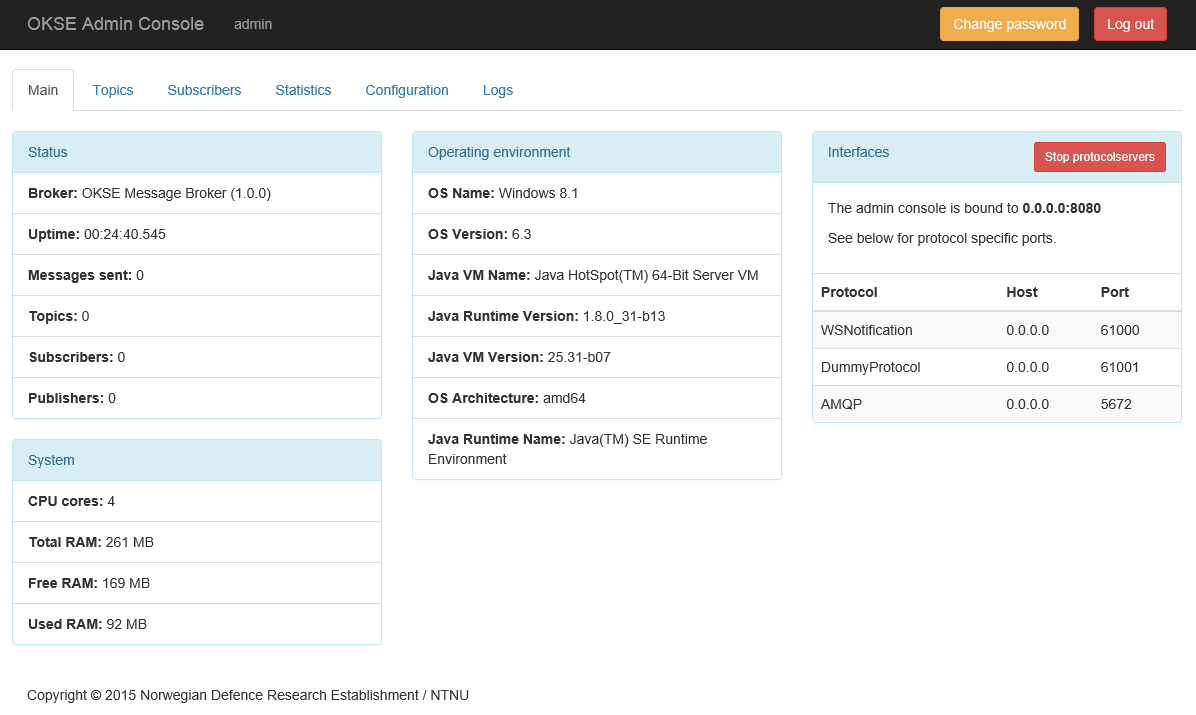
\includegraphics[width=\textwidth]{fig/oac/mainpane.png}}
    \caption{The OKSE Admin Console - Main pane} 
    \label{fig:OKSE Admin Console - Main pane}
  \end{figure}
\end{center}

\subsection{The Topics pane}
The Topics pane contains all the registered topics in OKSE. For each topic it is possible to see how many clients are subscribing to the topic (---comment about xpath not being subscribers??---). It is also possible to delete all topics or a specific topic. The 'Stop refresh'-button stops the automatic refreshing of the topic list. This can be use full when there are many new topic are generated, and you do not want the list to update (ex: you want to search in the list)

\begin{center}
  \begin{figure}[ht!]
    \makebox[\textwidth]{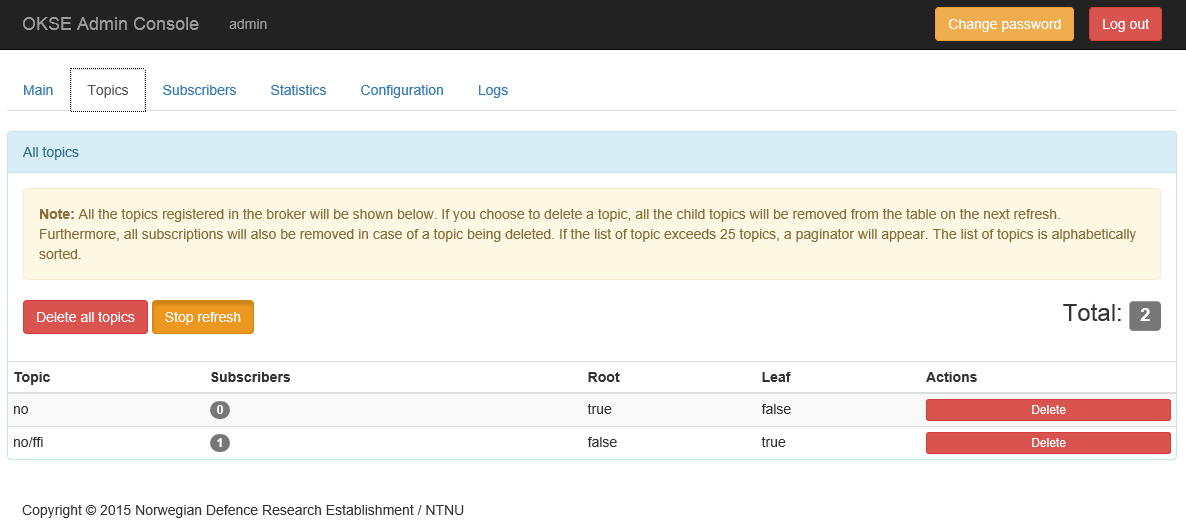
\includegraphics[width=\textwidth]{fig/oac/topicspane.png}}
    \caption{The OKSE Admin Console - Topics pane} 
    \label{fig:OKSE Admin Console - Topics pane}
  \end{figure}
\end{center}

\subsection{The Subscribers pane}
The subscribers pane shows all the subscribers (hosts). It also lists which protocol the subscriber are using, on which port, and if any filters are specified. One or all users can be deleted, denoted as unsubscribe in WSN and disconnect in AMQP. The 'Stop refresh'-button stops the automatic refreshing of the subscription list. This can be use full when there are many clients subscribing and/or unsubscribing, and you do not want the list to update (ex: you want to search in the list)

\begin{center}
  \begin{figure}[ht!]
    \makebox[\textwidth]{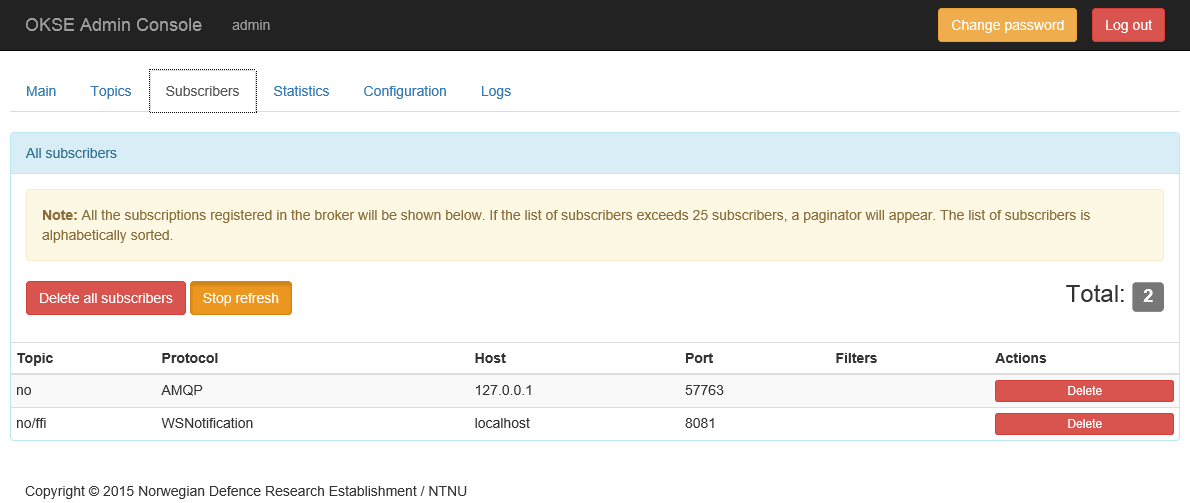
\includegraphics[width=\textwidth]{fig/oac/subscriptionspane.png}}
    \caption{The OKSE Admin Console - Subscriptions pane} 
    \label{fig:OKSE Admin Console - Subscriptions pane}
  \end{figure}
\end{center}

\subsection{The Statistics pane}
The Statistics pane prvides a list of protocol servers with statistics per protocol and total usage. "Sent" denotes the amount of messages sent on the different protocols. "Received" denotes messages received on current protocol. "Requests" are the total amount of requests on the protocol. The WSNotification protocol server "Requests" are subscribe request, message sendt to the broker, publisher registration, and trying to acccess an endpoint address. For AMQP a request are countet when the broker got a socket connection, and when a message is sendt to the broker. "Bad request" on the WSNotification protocol server can be trying to access an WSNotification endpoint. (---her---). Errors (---Her---). In the usage panel you get the total stats for all protocols.

\begin{center}
  \begin{figure}[ht!]
    \makebox[\textwidth]{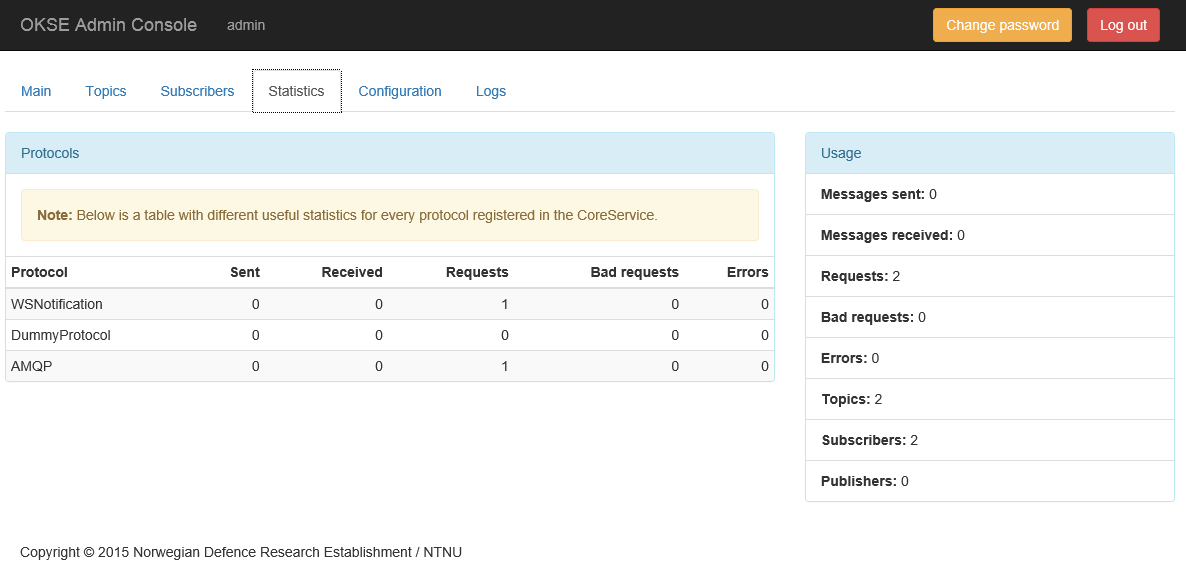
\includegraphics[width=\textwidth]{fig/oac/statisticspane.png}}
    \caption{The OKSE Admin Console - Statistics pane} 
    \label{fig:OKSE Admin Console - Statistics pane}
  \end{figure}
\end{center}

\subsection{The Configuration pane}
The Configuration pane have three sections; options, topic mapping and relays. In the option section you can change the auto update interval for refreshing the web page. The "Use AMQP queues instead of pub/sub topics" changes the queue semantic.

In the topic mapping section one can manually map from one topic to another one. The mapping is an asynchronous action. If a mapping is made between topic A and B, messages sent to A will also be forwarded to topic B. Messages sent to topic B will not be forwarded to topic A.

\begin{center}
  \begin{figure}[ht!]
    \makebox[\textwidth]{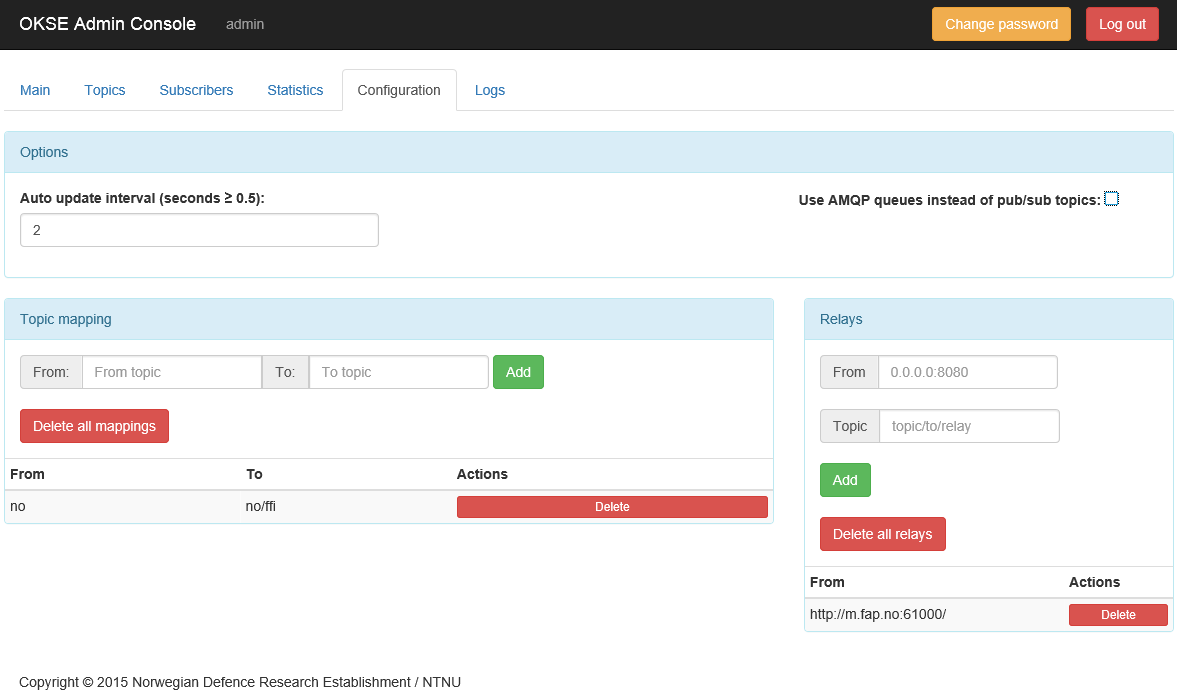
\includegraphics[width=\textwidth]{fig/oac/configurationpane.png}}
    \caption{The OKSE Admin Console - Configurations pane} 
    \label{fig:OKSE Admin Console - Configurations pane}
  \end{figure}
\end{center}

\subsection{The Logs pane}
The main feature of the "Logs" pane is the large text area, providing all of the information printed from the application. Logging is separated into 4 levels, "ERROR", "WARN", "INFO" and "DEBUG". The "DEBUG" level shows the full set of messages printed during system runtime. "INFO" prints messages that are meant to show the progress and events happening in the application. The "WARN" level prints messages that might potentially lead to system failure. Finally, "ERROR" shows events which has caused a failure in the system. There are one button for each of the message types, allowing the user to filter out information. The "Lines" area, lets the user decide how many lines of information that are displayed. Lastly, the "Stop refresh" buttons stops new messages from showing up in the text-area.

\begin{center}
  \begin{figure}[ht!]
    \makebox[\textwidth]{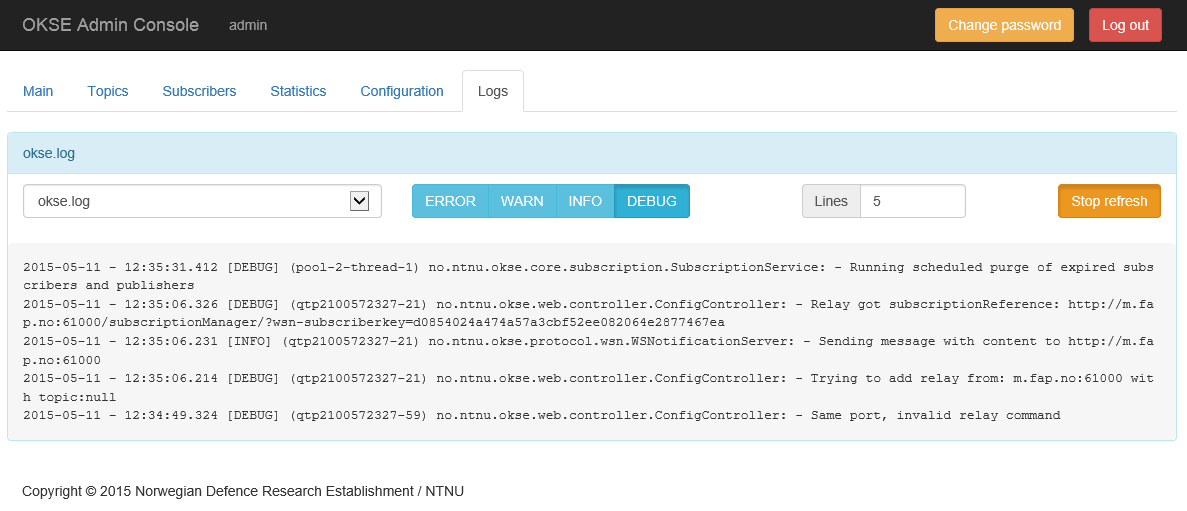
\includegraphics[width=\textwidth]{fig/oac/logpane.png}}
    \caption{The OKSE Admin Console - Logs pane} 
    \label{fig:OKSE Admin Console - Logs pane}
  \end{figure}
\end{center}

\section{Sending and receiving messages}

If you want to send a WSNotification message to OKSE you just send a valid WSNotification messages on a topic of your choice. OKSE will then distribute the message to all subscribers on the topic. If the topic does not exists OKSE will create it. To receive a WSNotification message you have to subscribe on a topic. You will then get all messages sent to the broker on the topic you subscribe on, regardless of witch protocol i originated from. For AMQP you have to connect to OKSE before you can send a AMQP message. The same applies to receive a message. To receive you also have to subscribe to a topic. 

The OKSE project does not contain any clients for sending and receiving messages, as the broker itself is the scope. Thus, additional software is required, in order to use the functionality of the broker itself. For testing purposeses a python script is included(bullrider.py) meant for sending valid WSNotification messages, and a java client to receive AMQP messages(AMQPreceive.jar).

\section{Configuration files}
\label{sec:configuration-files}
OKSE has three configurations files. The main configuration file is the okse.properties file. You also got log4j.properties, and topicmapping.properties. This chapter describe the default configuration.

\subsection{okse.properties}
\label{subsec:okse.properties}
 
 This is the main configuration file within the system. See below for a detailed list of all possible settings, and their description.

\begin{description}
\setlength{\itemsep}{0cm}%
  \item[sprint.application.name] \hfill \\
  Application name to be displayed in the Admin Console \hfill \\ Default: \verb!OKSE Message Broker!
  \item[server.port] \hfill \\
  Tells Jetty which port the Admin Console should use \hfill \\ Default: \verb!8080!
  \item[ADMIN\_PANEL\_HOST] \hfill \\
  The host the Admin Console should use \hfill \\ Default: \verb!0.0.0.0!
  \item[CACHE\_MESSAGES] \hfill \\
  Tells OKSE if it should cache messages \hfill \\ Default: \verb!true!
  \item[BROADCAST\_SYSTEM\_MESSAGES\_TO\_SUBSCRIBERS] \hfill \\
  Tells OKSE if system messages shoudl be broadcasted to all subscribers \hfill \\ Default: \verb!false!
  \item[ENABLE\_WSNU\_DEBUG\_OUTPUT] \hfill \\
  Tells OKSE if it should log WSNU \hfill \\ Default: \verb!false!
  \item[DEFAULT\_SUBSCRIPTION\_TERMINATION\_TIME] \hfill \\
  Tells OKSE what the subscription termination time should be \hfill \\ Default: \verb!15552000000!
  \item[DEFAULT\_PUBLISHER\_TERMINATION\_TIME] \hfill \\
  Tells OKSE what the publisher termination time should be \hfill \\ Default: \verb!15552000000!
  \item[TOPIC\_MAPPING] \hfill \\
  Tells OKSE the path to the topic mapping configuration file \hfill \\ Default: \verb!config/topicmapping.properties!
  \item[WSN\_HOST] \hfill \\
  Tells OKSE what host WSNotificanServer should listen to \hfill \\ Default: \verb!0.0.0.0!
  \item[WSN\_PORT] \hfill \\
  Tells OKSE what port WSNotificationServer should listen to \hfill \\ Default: \verb!61000!
  \item[WSN\_CONNECTION\_TIMEOUT] \hfill \\
  Tells OKSE what connection timeout to use with WS-Notification \hfill \\ Default: \verb!5!
  \item[WSN\_POOL\_SIZE] \hfill \\
   WSNotification http client thread pool used to queue outbound requests \hfill \\ Default: \verb!50!
   \item[WSN\_MESSAGE\_CONTENT\_ELEMENT\_NAME] \hfill \\
  Tells OKSE what name non-XML content should be wrapped in \hfill \\ Default: \verb!Content!
  \item[WSN\_USES\_NAT] \hfill \\
  Tells OKSE if it's hosted behind NAT/Port forwarded network \hfill \\ Default: \verb!false!
  \item[WSN\_WAN\_HOST] \hfill \\
  Tells OKSE what host it's behind when using NAT \hfill \\ Default: \verb!test.doman.com!
  \item[WSN\_WAN\_PORT] \hfill \\
  Tells OKSE what port it's behind when using NAT \hfill \\ Default: \verb!61000!
  \item[DUMMYPROTOCOL\_HOST] \hfill \\
  Tells OKSE what host DummyProtocolServer should listen to \hfill \\ Default: \verb!0.0.0.0!
  \item[DUMMYPROTOCOL\_PORT] \hfill \\
  Tells OKSE what port DummyProtocolServer should listen to \hfill \\ Default: \verb!61001!
  \item[AMQP\_HOST] \hfill \\
  Tells OKSE what host AMQPProtocolServer should listen to \hfill \\ Default: \verb!0.0.0.0!
  \item[AMQP\_PORT] \hfill \\
  Tells OKSE what port AMQPProtocolServer should listen to \hfill \\ Default: \verb!5672!
  \item[AMQP\_USE\_QUEUE] \hfill \\
  Tells OKSE if AMQP should use the standard queue or the non-standard topic implementation \hfill \\ Default: \verb!false!
  \item[AMQP\_USE\_SASL] \hfill \\
  Tells OKSE if AMQP should use SASL \hfill \\ Default: \verb!true!
  \item[spring.resources.cache-period] \hfill \\
  Tells Spring what cache-period to set on HTTP-requests \hfill \\ Default: \verb!1!
  \item[spring.thymeleaf.suffix] \hfill \\
  Tells Spring what all Thymeleaf templates are suffixed with \hfill \\ Default: \verb!.html! 
   \item[spring.thymeleaf.mode] \hfill \\
  Tells Spring what type all Thymeleaf templates are \hfill \\ Default: \verb!HTML5!
   \item[spring.thymeleaf.encoding] \hfill \\
  Tells Spring what encoding to use on all Thymeleaf templates \hfill \\ Default: \verb!UTF-8!
   \item[spring.thymeleaf.content-type] \hfill \\
  Tells Spring what content-type all Thymeleaf templates should be returned with \hfill \\ Default: \verb!text/html! 
\end{description}
  
 \subsection{log4j.properties}
 \label{subsec:log4j.properties}
 
This is the configuration file for all the log files available for the system. See below for a detailed list of all possible settings, and their description.

\begin{description}

\setlength{\itemsep}{0cm}%
  \item[log] \hfill \\
  Default folder location for log files, relative to .jar file \hfill \\ Default: \verb!logs!
  \item[pattern] \hfill \\
  Default pattern to print log output in \hfill \\ Default: \verb!%d{yyyy-MM-dd - HH:mm:ss.SSS} [%p] (%t) %c: - %m%n!
   \item[maxLogFileSize] \hfill \\
  Max log file size, before log rotate \hfill \\ Default: \verb!5MB!
   \item[numberOfBackups] \hfill \\
  Max number of log files, before it purges old files \hfill \\ Default: \verb!10!
   \item[log4j.logger.no.ntnu.okse] \hfill \\
  Default log level for okse log messages \hfill \\ Default: \verb!DEBUG, OKSE!
  \item[log4j.logger.org.apache.qpid] \hfill \\
  Default log level for qpid log messages \hfill \\ Default: \verb!DEBUG, QPID!
  \item[log4j.logger.org.eclipse.jetty] \hfill \\
  Default log level for Jetty log messages \hfill \\ Default: \verb!INFO, JETTY!
  \item[log4j.logger.org.springframework] \hfill \\
  Default log level for Spring log messages \hfill \\ Default: \verb!INFO, SPRING!
  
  \item[log4j.appender.OKSE] \hfill \\
  Default appender to use for OKSE logs \hfill \\ Default: \verb!org.apache.log4j.RollingFileAppender!
  \item[log4j.appender.OKSE.File] \hfill \\
  Default log file to use for OKSE logs \hfill \\ Default: \verb!${log}/okse.log!
   \item[log4j.appender.OKSE.MaxFileSize] \hfill \\
  Default log file size to use for OKSE logs \hfill \\ Default: \verb!${maxLogFileSize}!
   \item[log4j.appender.OKSE.MaxBackupIndex] \hfill \\
  Number of backups for OKSE logs \hfill \\ Default: \verb!${numberOfBackups}!
   \item[log4j.appender.OKSE.layout] \hfill \\
  Pattern engine for OKSE logs \hfill \\ Default: \verb!org.apache.log4j.PatternLayout!
   \item[log4j.appender.OKSE.layout.conversionPattern] \hfill \\
  Default pattern to use for OKSE logs \hfill \\ Default: \verb!${Pattern}!

    \item[log4j.appender.SPRING] \hfill \\
  Default appender to use for SPRING logs \hfill \\ Default: \verb!org.apache.log4j.RollingFileAppender!
  \item[log4j.appender.SPRING.File] \hfill \\
  Default log file to use for SPRING logs \hfill \\ Default: \verb!${log}/spring.log!
   \item[log4j.appender.SPRING.MaxFileSize] \hfill \\
  Default log file size to use for SPRING logs \hfill \\ Default: \verb!${maxLogFileSize}!
   \item[log4j.appender.SPRING.MaxBackupIndex] \hfill \\
  Number of backups for SPRING logs \hfill \\ Default: \verb!${numberOfBackups}!
   \item[log4j.appender.SPRING.layout] \hfill \\
  Pattern engine for SPRING logs \hfill \\ Default: \verb!org.apache.log4j.PatternLayout!
   \item[log4j.appender.SPRING.layout.conversionPattern] \hfill \\
  Default pattern to use for SPRING logs \hfill \\ Default: \verb!${Pattern}!

  \item[log4j.appender.JETTY] \hfill \\
  Default appender to use for JETTY logs \hfill \\ Default: \verb!org.apache.log4j.RollingFileAppender!
  \item[log4j.appender.JETTY.File] \hfill \\
  Default log file to use for JETTY logs \hfill \\ Default: \verb!${log}/okse.log!
   \item[log4j.appender.JETTY.MaxFileSize] \hfill \\
  Default log file size to use for JETTY logs \hfill \\ Default: \verb!${maxLogFileSize}!
   \item[log4j.appender.JETTY.MaxBackupIndex] \hfill \\
  Number of backups for JETTY logs \hfill \\ Default: \verb!${numberOfBackups}!
   \item[log4j.appender.JETTY.layout] \hfill \\
  Pattern engine for JETTY logs \hfill \\ Default: \verb!org.apache.log4j.PatternLayout!
   \item[log4j.appender.JETTY.layout.conversionPattern] \hfill \\
  Default pattern to use for JETTY logs \hfill \\ Default: \verb!${Pattern}!
  
    \item[log4j.appender.QPID] \hfill \\
  Default appender to use for QPID logs \hfill \\ Default: \verb!org.apache.log4j.RollingFileAppender!
  \item[log4j.appender.QPID.File] \hfill \\
  Default log file to use for QPID logs \hfill \\ Default: \verb!${log}/qpid.log!
   \item[log4j.appender.QPID.MaxFileSize] \hfill \\
  Default log file size to use for QPID logs \hfill \\ Default: \verb!${maxLogFileSize}!
   \item[log4j.appender.QPID.MaxBackupIndex] \hfill \\
  Number of backups for QPID logs \hfill \\ Default: \verb!${numberOfBackups}!
   \item[log4j.appender.QPID.layout] \hfill \\
  Pattern engine for QPID logs \hfill \\ Default: \verb!org.apache.log4j.PatternLayout!
   \item[log4j.appender.QPID.layout.conversionPattern] \hfill \\
  Default pattern to use for QPID logs \hfill \\ Default: \verb!${Pattern}!

 \item[log4j.appender.stdout] \hfill \\
  Default appender to use for console output \hfill \\ Default: \verb!org.apache.log4j.ConsoleAppender!
   \item[log4j.appender.stdout.Target] \hfill \\
  Default target to use for console output \hfill \\ Default: \verb!System.out!
    \item[log4j.appender.stdout.layout] \hfill \\
  Pattern engine for console logs \hfill \\ Default: \verb!org.apache.log4j.PatternLayout!
   \item[log4j.appender.stdout.layout.conversionPattern] \hfill \\
  Default pattern to use for console logs \hfill \\ Default: \verb!${Pattern}!
  
 \end{description}
 
 \subsection{topicmapping.properties}
 \label{subsec:topicmapping.properties}
 
 This is a configuration file for adding predefined topic mappings to be available when the broker boots. The mapping is asyncron. This means that the broker forward messages from one topic to another one, but not back again (TopicA forward to TopicB, but not visa versa). If you want syncron forwarding (A to B, and B to A), you have to add two mappings, A=B and B=A. By default, there are no topic mapping listed. To add predefined topic mappings, use the following format: \verb!from=to!. An example mapping is: \verb!no/ffi=nato/hq/info!.
This will forward all messages recevived on no/ffi to nato/hq/info
 
\section{Troubleshooting}

If you encounter any problems with the software, check the following points before you contact the development team: 

\begin{itemize}
\setlength{\itemsep}{0cm}%
\item Do you have the correct JRE? For OKSE Message Broker to run properly, you need version 8 or newer. Other versions than this may cause problems, or not work at all.
\item Network connectivity. Verify that your network connection is working and that the ports are open. Also ensure that you use port forwarding if you don't have a public IP. 
\end{itemize}

\clearpage